\documentclass[a4paper,14pt]{article}


% настройка языка 
\usepackage[utf8]{inputenc}
\usepackage[english, russian]{babel}

% настройка параметров листа
\usepackage[height=297mm, width=210mm, left=3cm, top=2cm, right=1cm, bottom=3cm]{geometry}

% добавление надписей и картинок на фон
\usepackage{eso-pic}

% получение кол-ва листов в файле
\usepackage{lastpage}

% для добавления надписей в рамку
\usepackage[absolute,overlay]{textpos}

% изменение формата номера figure
\usepackage{amsmath}

% настройка подписей к картинкам и таблицам
\usepackage{caption}

% добавляет отступ к 1-ому абзацу после раздела
\usepackage{indentfirst} 

% работа с таблицами
\usepackage{tabularx}

% добавление гиперссылок
\usepackage{hyperref}

% работа с изображениями
\usepackage{graphicx}

% работа с позицией для figure
\usepackage{float}

% добавление предварительных вычислений перед выводом в файл
\usepackage{calc}

% добавление картинок в качестве фона
\usepackage{background}

% Устанавливает тире между номером и текстом
\usepackage[justification=centering]{caption}

\usepackage{titlesec}


\captionsetup{labelsep=endash}

\captionsetup[figure]{name={Рисунок},labelsep=endash} 
\captionsetup[table]{name={Таблица},labelsep=endash} 

\numberwithin{figure}{section}
\numberwithin{table}{section}

\setlength{\parindent}{12.5mm} 

\titleformat{\subsubsection}{\large\bfseries}{\thesubsubsection}{1em}{}

\newcommand{\chipher}{
        {\fontsize{16pt}{16pt}\selectfont  КР.ИИ-21.210563-3 81 00}
}

\newcommand{\theme}{Разработка мобильного приложения для опредления эмоций человека}

\newcommand{\student}{Худик А.А.}

\newcommand{\teacher}{Кулеша В.И.}


\begin{document}

        \backgroundsetup{
                scale=3,
                color=black,
                opacity=0.1,
                angle=0,
                position=current page.south,
                vshift=5cm,
                hshift=0cm,
                contents={}
        }
        \setcounter{page}{2}
        \pagestyle{empty}


        \renewcommand{\contentsname}{\centering \MakeUppercase{Содержание}}

        \newcommand{\titlePage}{

    \begin{center}
        МИНИСТЕРСТВО ОБРАЗОВАНИЯ РЕСПУБЛИКИ БЕЛАРУСЬ \\
        УЧРЕЖДЕНИЕ ОБРАЗОВАНИЯ \\
        <<БРЕСТСКИЙ ГОСУДАРСТВЕННЫЙ ТЕХНИЧЕСКИЙ УНИВЕРСИТЕТ>> \\
        ФАКУЛЬТЕТ ЭЛЕКТРОННО-ИНФОРМАЦИОННЫХ СИСТЕМ \\
        Кафедра интеллектуальных информационных технологий \\[4cm]
        
            \MakeUppercase{
                {\bf Пояснительная записка \\}
                к курсовой работе по дисциплине \\
            }
        
            <<Технологии и инструментальные средства проектирования интеллектуальных систем>> \\
            Тема: <<\theme>> 
            \\[.5cm]
            
            \chipher \\[4cm]
            
    \end{center}

    \begin{flushright}
        \begin{minipage}{0.35\textwidth}
            \begin{flushleft}
                Листов: \pageref{LastPage} \\[1cm]
                {\bf Выполнил:} \\
                студент 4 курса, \\
                ФЭИС, \\
                группы ИИ-21 \\
                \student \\
                {\bf Проверил:} \\
                \teacher
            \end{flushleft}
        \end{minipage}
    \end{flushright}

    \vfill 

    \begin{center}
        Брест \the\year
    \end{center}

    \newpage
}



        


\newcommand{\applicationTitlePage}{

    \begin{center}
        МИНИСТЕРСТВО ОБРАЗОВАНИЯ РЕСПУБЛИКИ БЕЛАРУСЬ \\
        УЧРЕЖДЕНИЕ ОБРАЗОВАНИЯ \\
        <<БРЕСТСКИЙ ГОСУДАРСТВЕННЫЙ ТЕХНИЧЕСКИЙ УНИВЕРСИТЕТ>> \\
        ФАКУЛЬТЕТ ЭЛЕКТРОННО-ИНФОРМАЦИОННЫХ СИСТЕМ \\
        Кафедра интеллектуальных информационных технологий \\[4cm]
        
         
            \MakeUppercase{
                {\bf Приложение А \\}
                
            }
            <<Текст программы>> \\[4cm]
        
           
            
        

    \end{center}

    \begin{flushright}
        \begin{minipage}{0.35\textwidth}
            \begin{flushleft}
                {\bf Выполнил:} \\
                студент 4-го курса, \\
                ФЭИС, \\
                группы ИИ-21 \\
                Худик А.А. \\
                {\bf Проверил:} \\
                Кулеша В.И.
            \end{flushleft}
        \end{minipage}
    \end{flushright}

    \vfill 

    \begin{center}
        Брест \the\year
    \end{center}

    \newpage

}



        \newcommand{\applicationContent}{
    Схема взаимодействия компонентов системы (рис. 1).
    \begin{figure}[H]
        \centering
        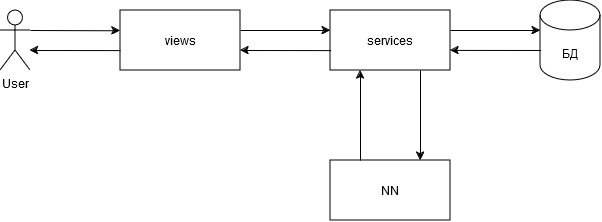
\includegraphics[width=0.8\textwidth]{application/components.png} 
        \caption{Схема взаимодействия компонентов системы}
    \end{figure}

    \newpage
    
    Схема обработки видео (рис. 2).
    \begin{figure}[H]
        \centering
        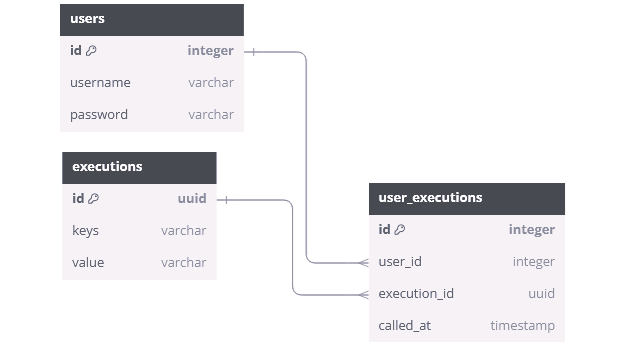
\includegraphics[width=0.8\textwidth]{application/DB-scheme.png} 
        \caption{Схема обработки видео}
    \end{figure}
}
        \newcommand{\contentTablePage}{
    
    % шифр
    \begin{textblock*}{12cm}(8.5cm,25.8cm) 
        \centering 
        \chipher
    \end{textblock*}    

    % лист 3
    \begin{textblock*}{1.5cm}(17cm,27.3cm) 
        \centering 
        3
    \end{textblock*}   

    % листов общее кол-во
    \begin{textblock*}{2cm}(18.5cm,27.3cm) 
        \centering 
        \pageref{LastPage}
    \end{textblock*}  
    
    % уо бргту
    \begin{textblock*}{5cm}(15.5cm,28.3cm) 
        \centering 
        УО <<БрГТУ>>
    \end{textblock*} 

    % тема работы
    \begin{textblock*}{7cm}(8.5cm,26.8cm) 
        \centering 
        \theme
    \end{textblock*} 

    % мое фио
    \begin{textblock*}{2.3cm}(3.74cm,26.85cm) 
        \centering 
        {\fontsize{9pt}{9pt}\selectfont \student}
    \end{textblock*} 

    % фио преподавателя
    \begin{textblock*}{2.3cm}(3.74cm,27.35cm) 
        \centering 
        {\fontsize{9pt}{9pt}\selectfont \teacher}
    \end{textblock*} 


    % вставляем рамку
    % \AddToShipoutPictureBG{

    %     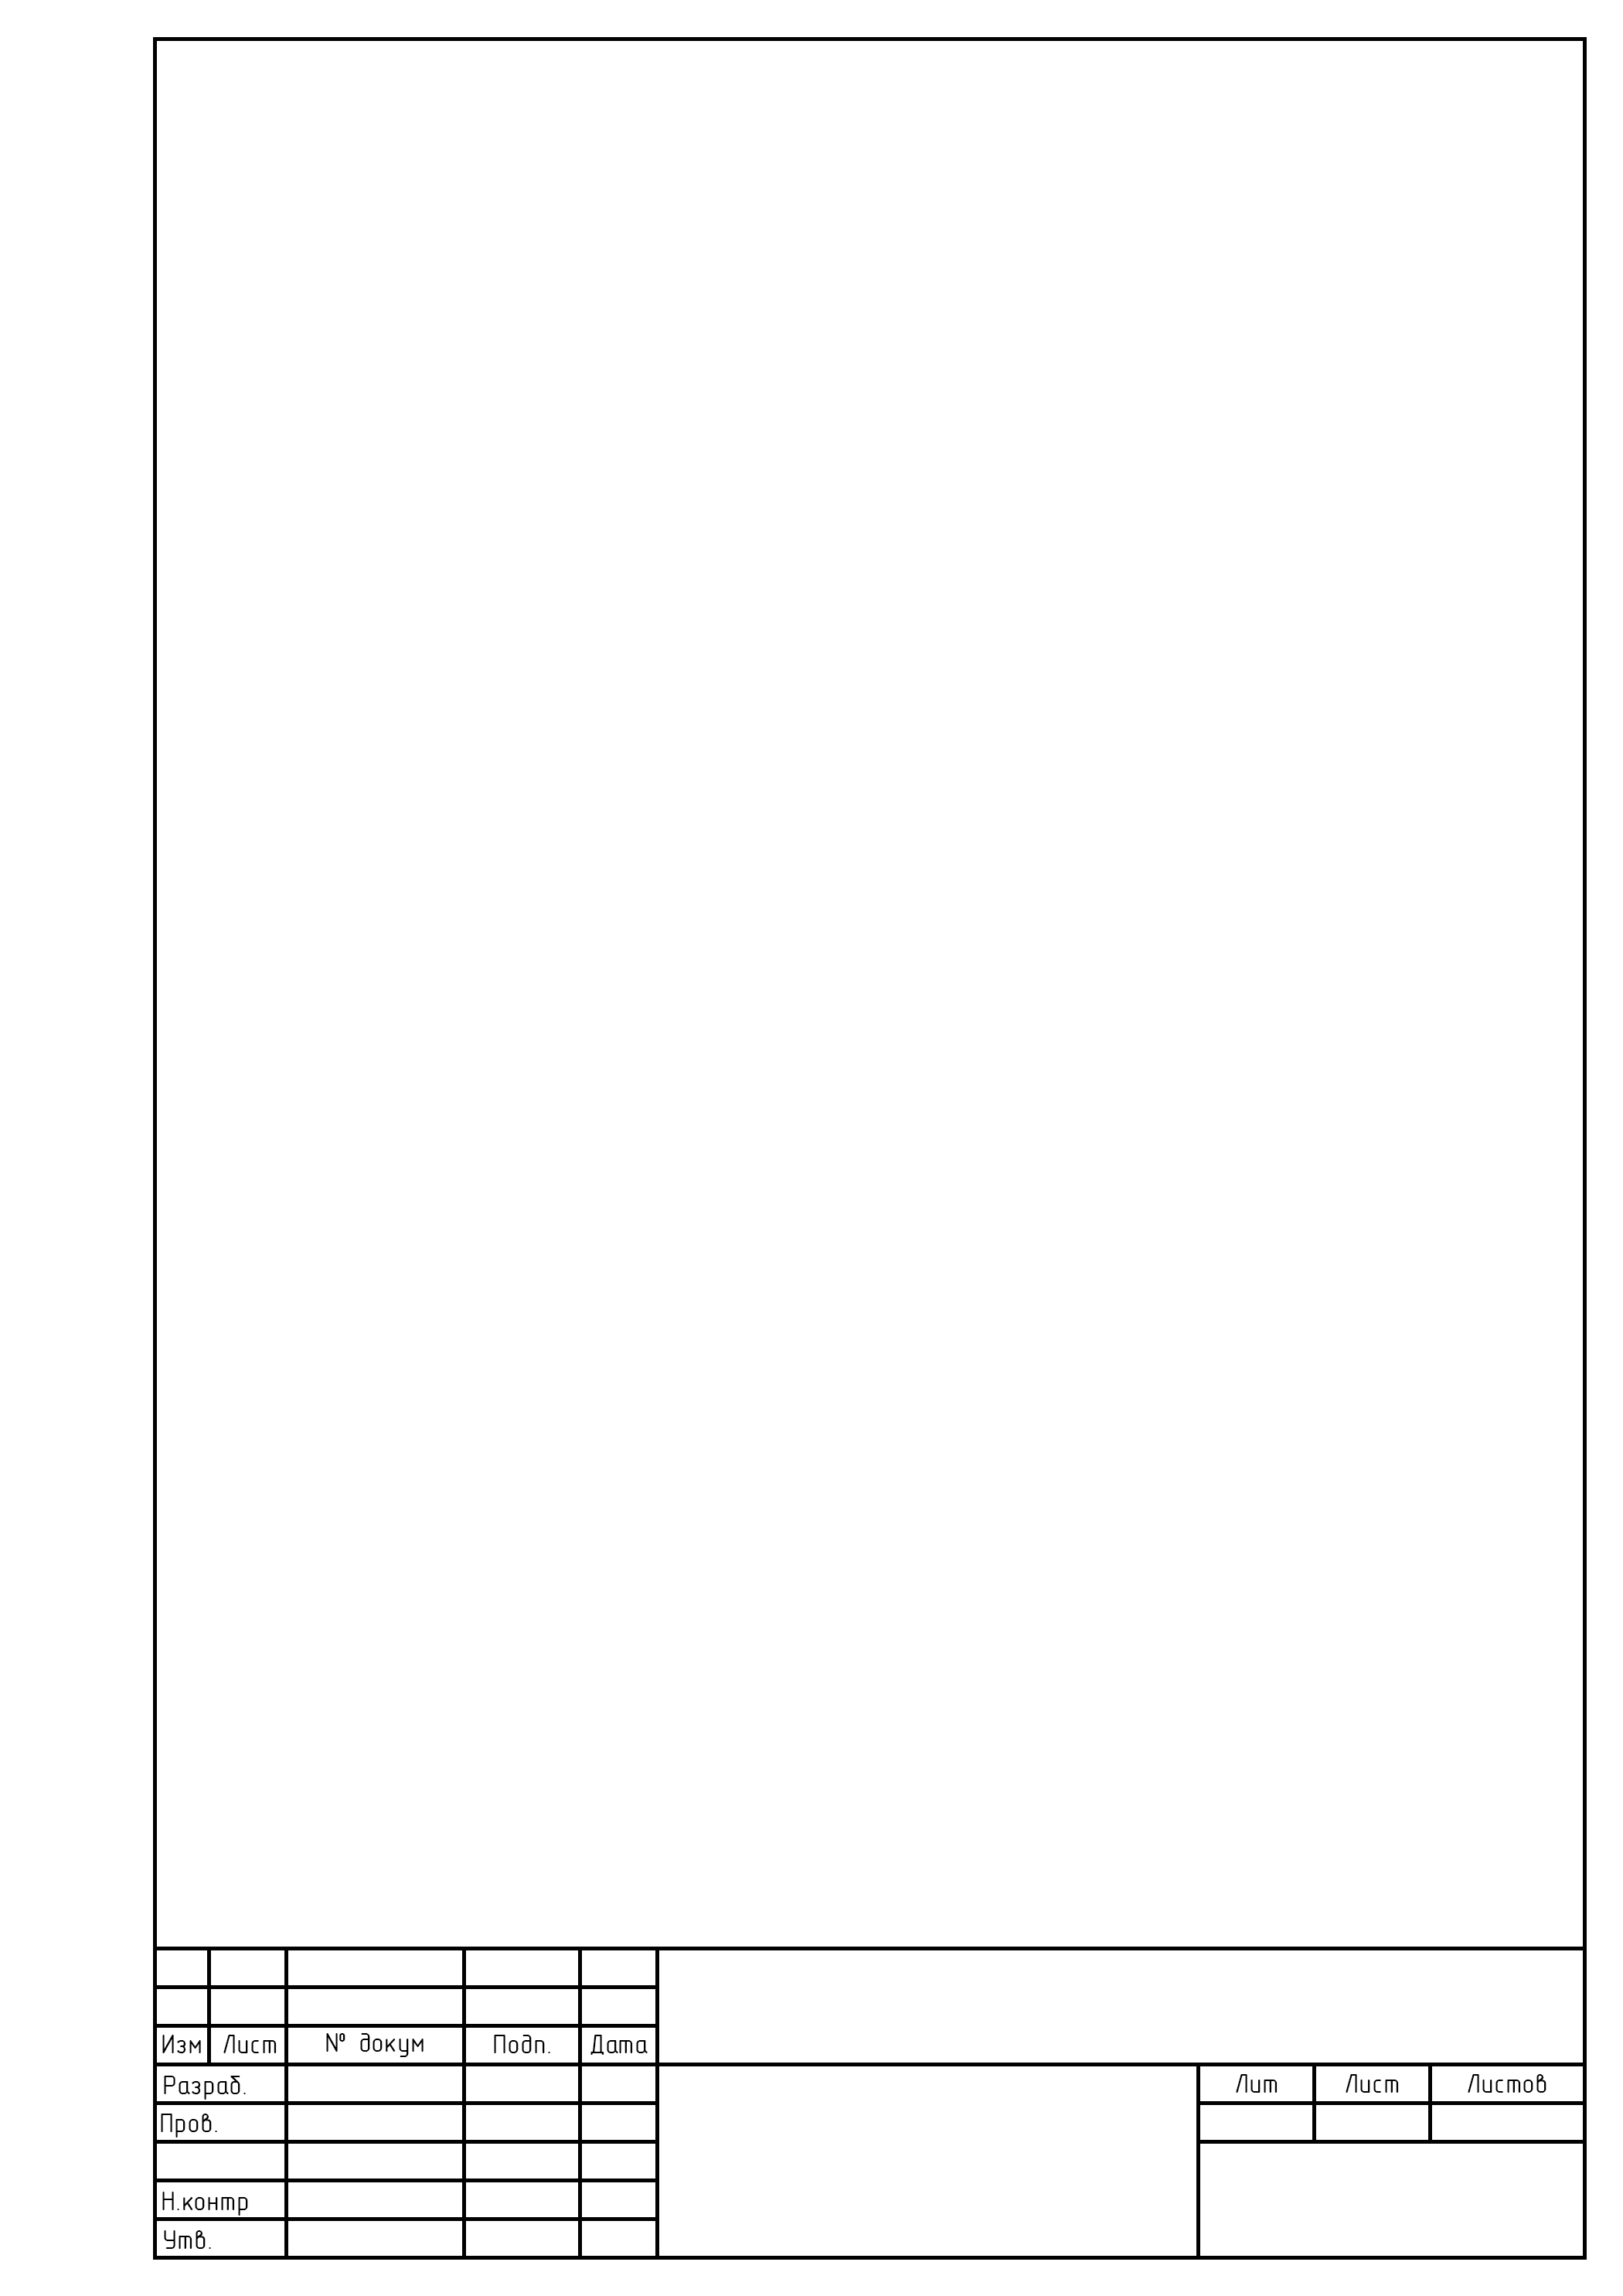
\includegraphics[width=\paperwidth,height=\paperheight]{border/border22.png}
    % }
    \backgroundsetup{
        scale=1,
        color=black,
        opacity=1,
        angle=0,
        position=current page.center,
        vshift=0cm, hshift=0cm,
        contents={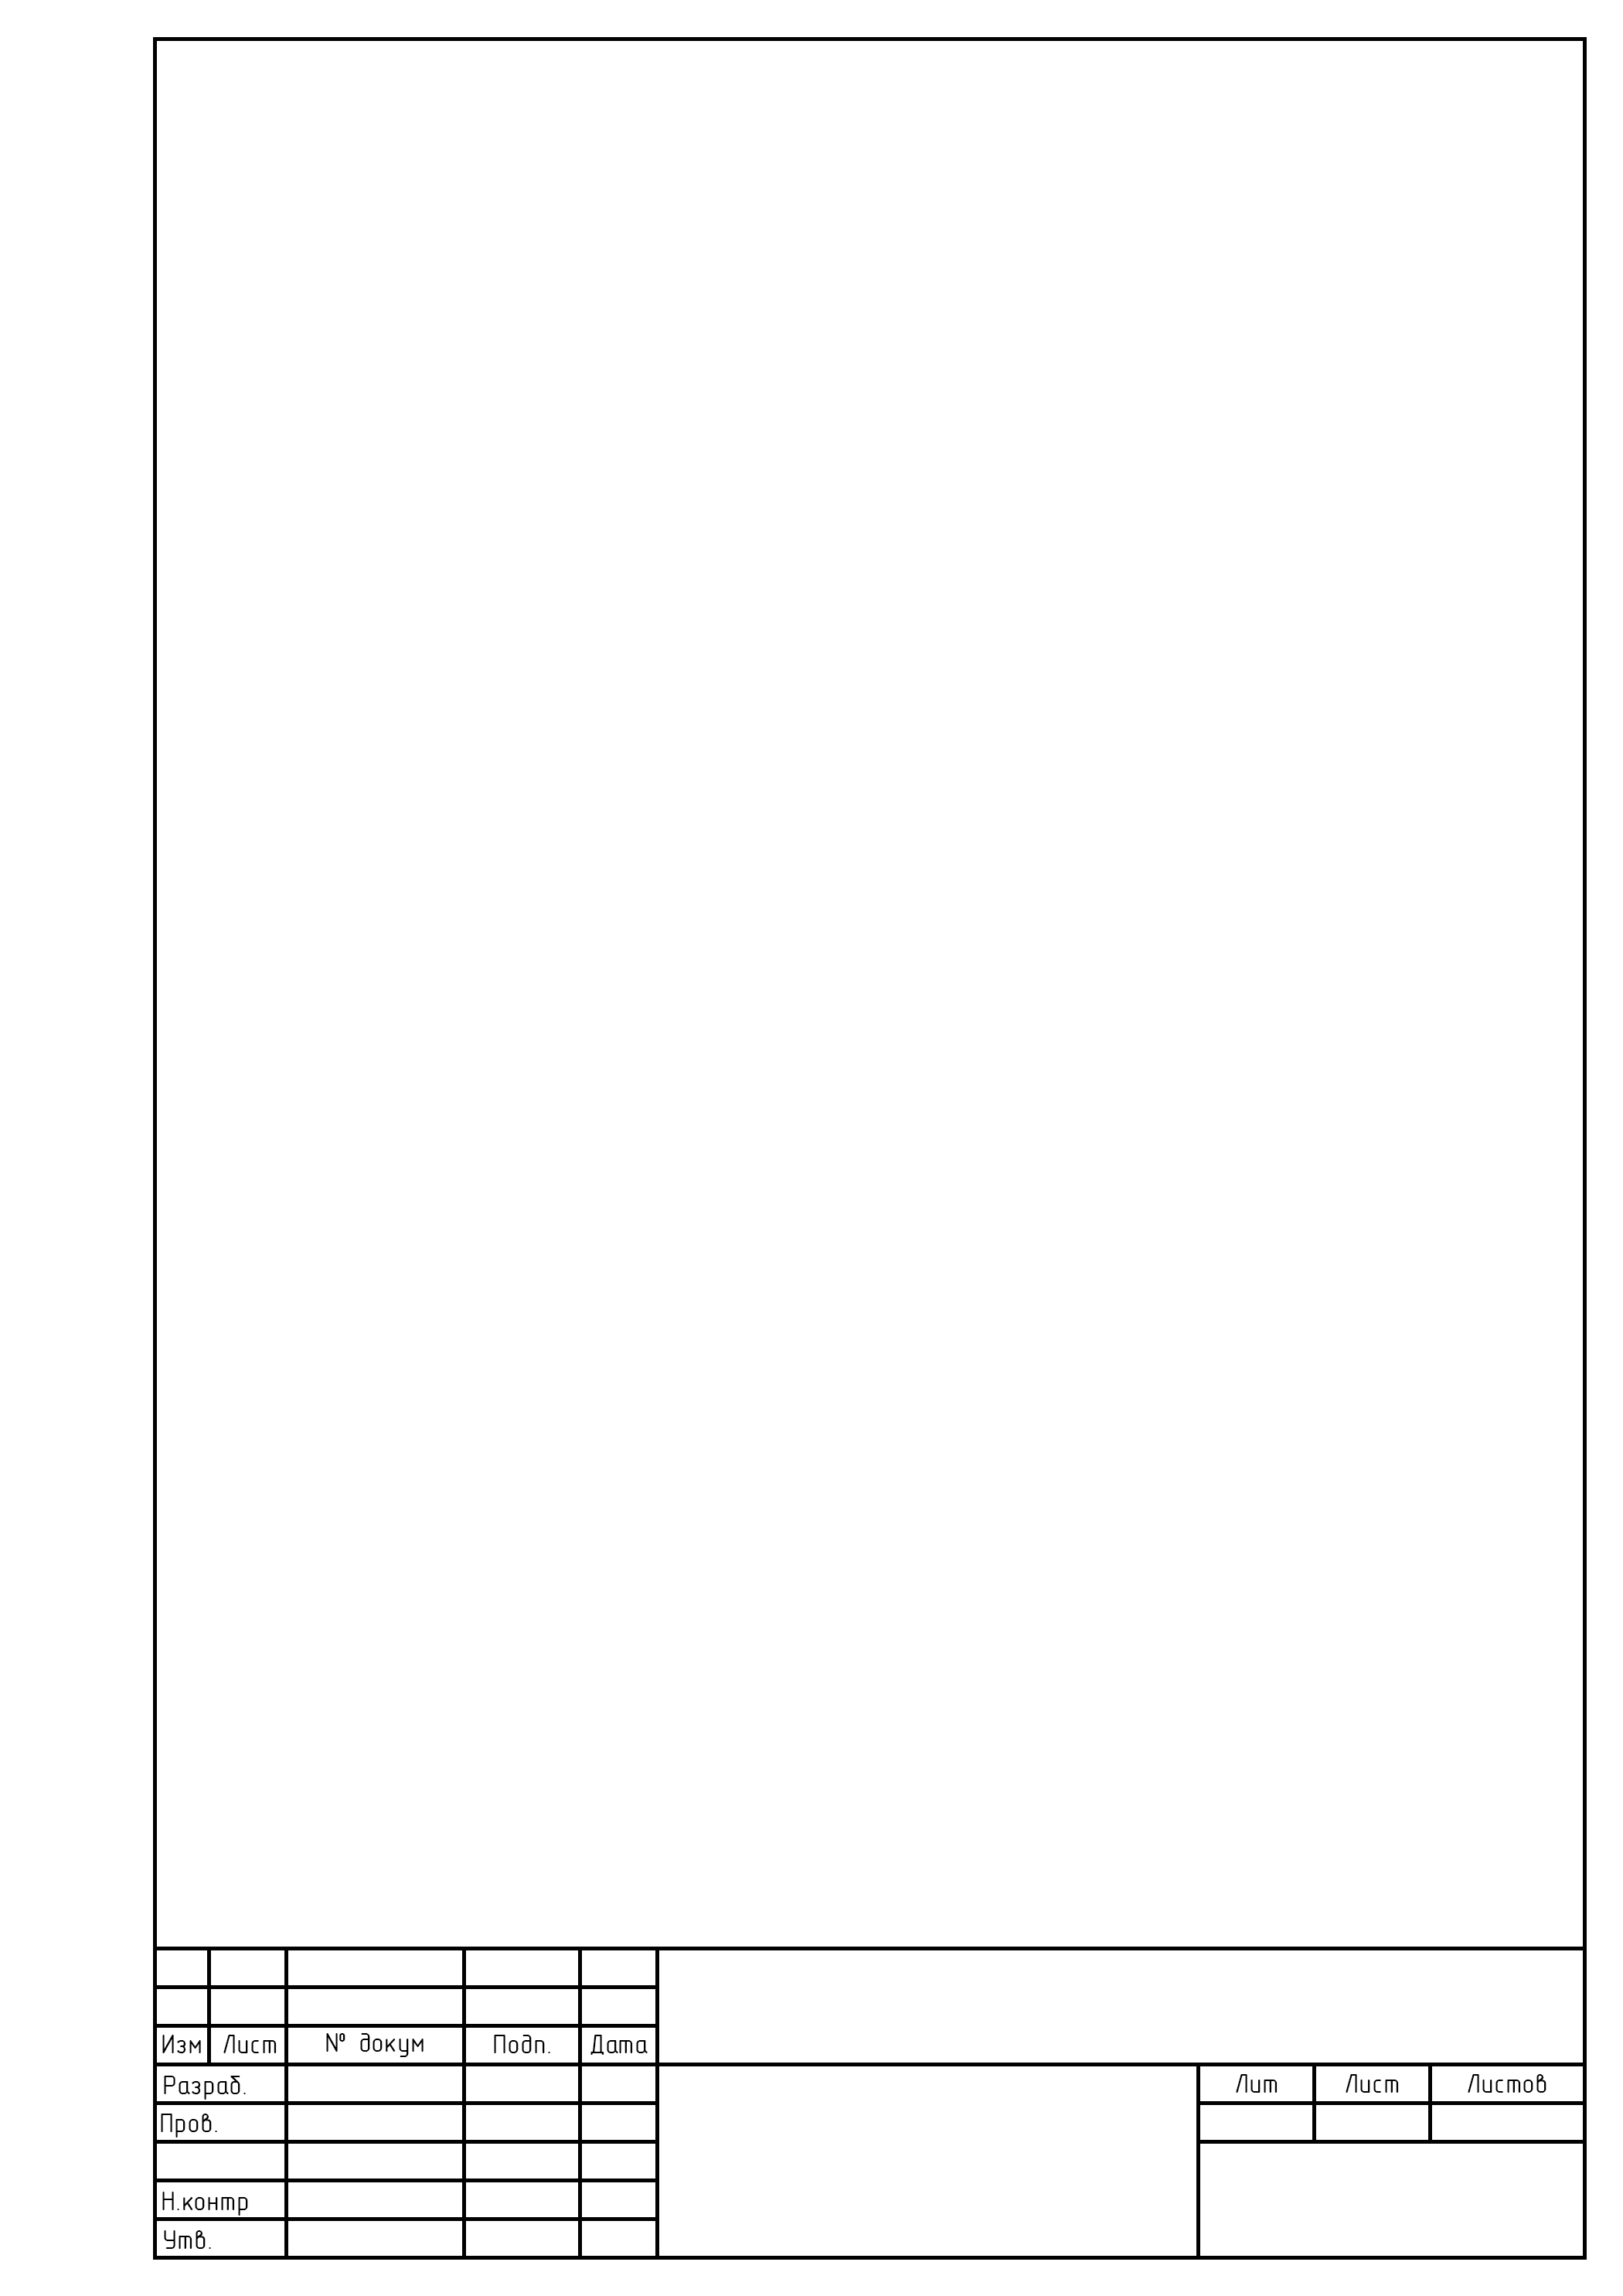
\includegraphics[width=\paperwidth,height=\paperheight]{border/border22.png}}
    }

    % номер для следующей страницы
    \AddToShipoutPicture{
                \begin{textblock*}{1cm}(19.5cm,28.6cm) 
                        \centering 
                        \number\numexpr\thepage+1\relax
                \end{textblock*}
        }
    
    % содержание
    \tableofcontents

    \newpage
    \ClearShipoutPicture

    \backgroundsetup{
                scale=3,
                color=black,
                opacity=0.1,
                angle=0,
                position=current page.south,
                vshift=5cm,
                hshift=0cm,
                contents={}
        }
}
        \newcommand{\applicationContent}{
    Схема взаимодействия компонентов системы (рис. 1).
    \begin{figure}[H]
        \centering
        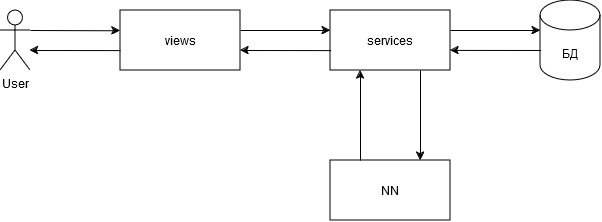
\includegraphics[width=0.8\textwidth]{application/components.png} 
        \caption{Схема взаимодействия компонентов системы}
    \end{figure}

    \newpage
    
    Схема обработки видео (рис. 2).
    \begin{figure}[H]
        \centering
        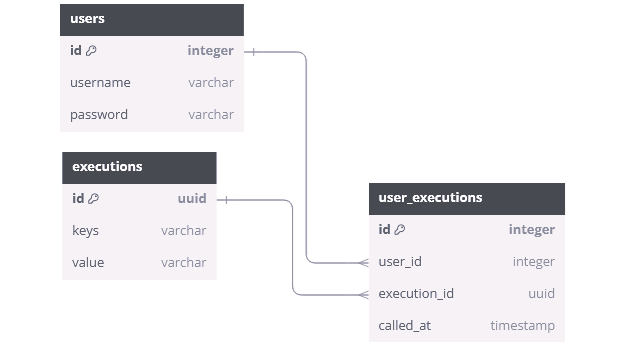
\includegraphics[width=0.8\textwidth]{application/DB-scheme.png} 
        \caption{Схема обработки видео}
    \end{figure}
}


        \fontsize{14}{17.5}\selectfont    
        
        \titlePage

        \contentTablePage

        % Устанавливаем картинку на фон
    \backgroundsetup{
        scale=1,
        color=black,
        opacity=1,
        angle=0,
        position=current page.center,
        vshift=0cm, hshift=0cm,
        contents={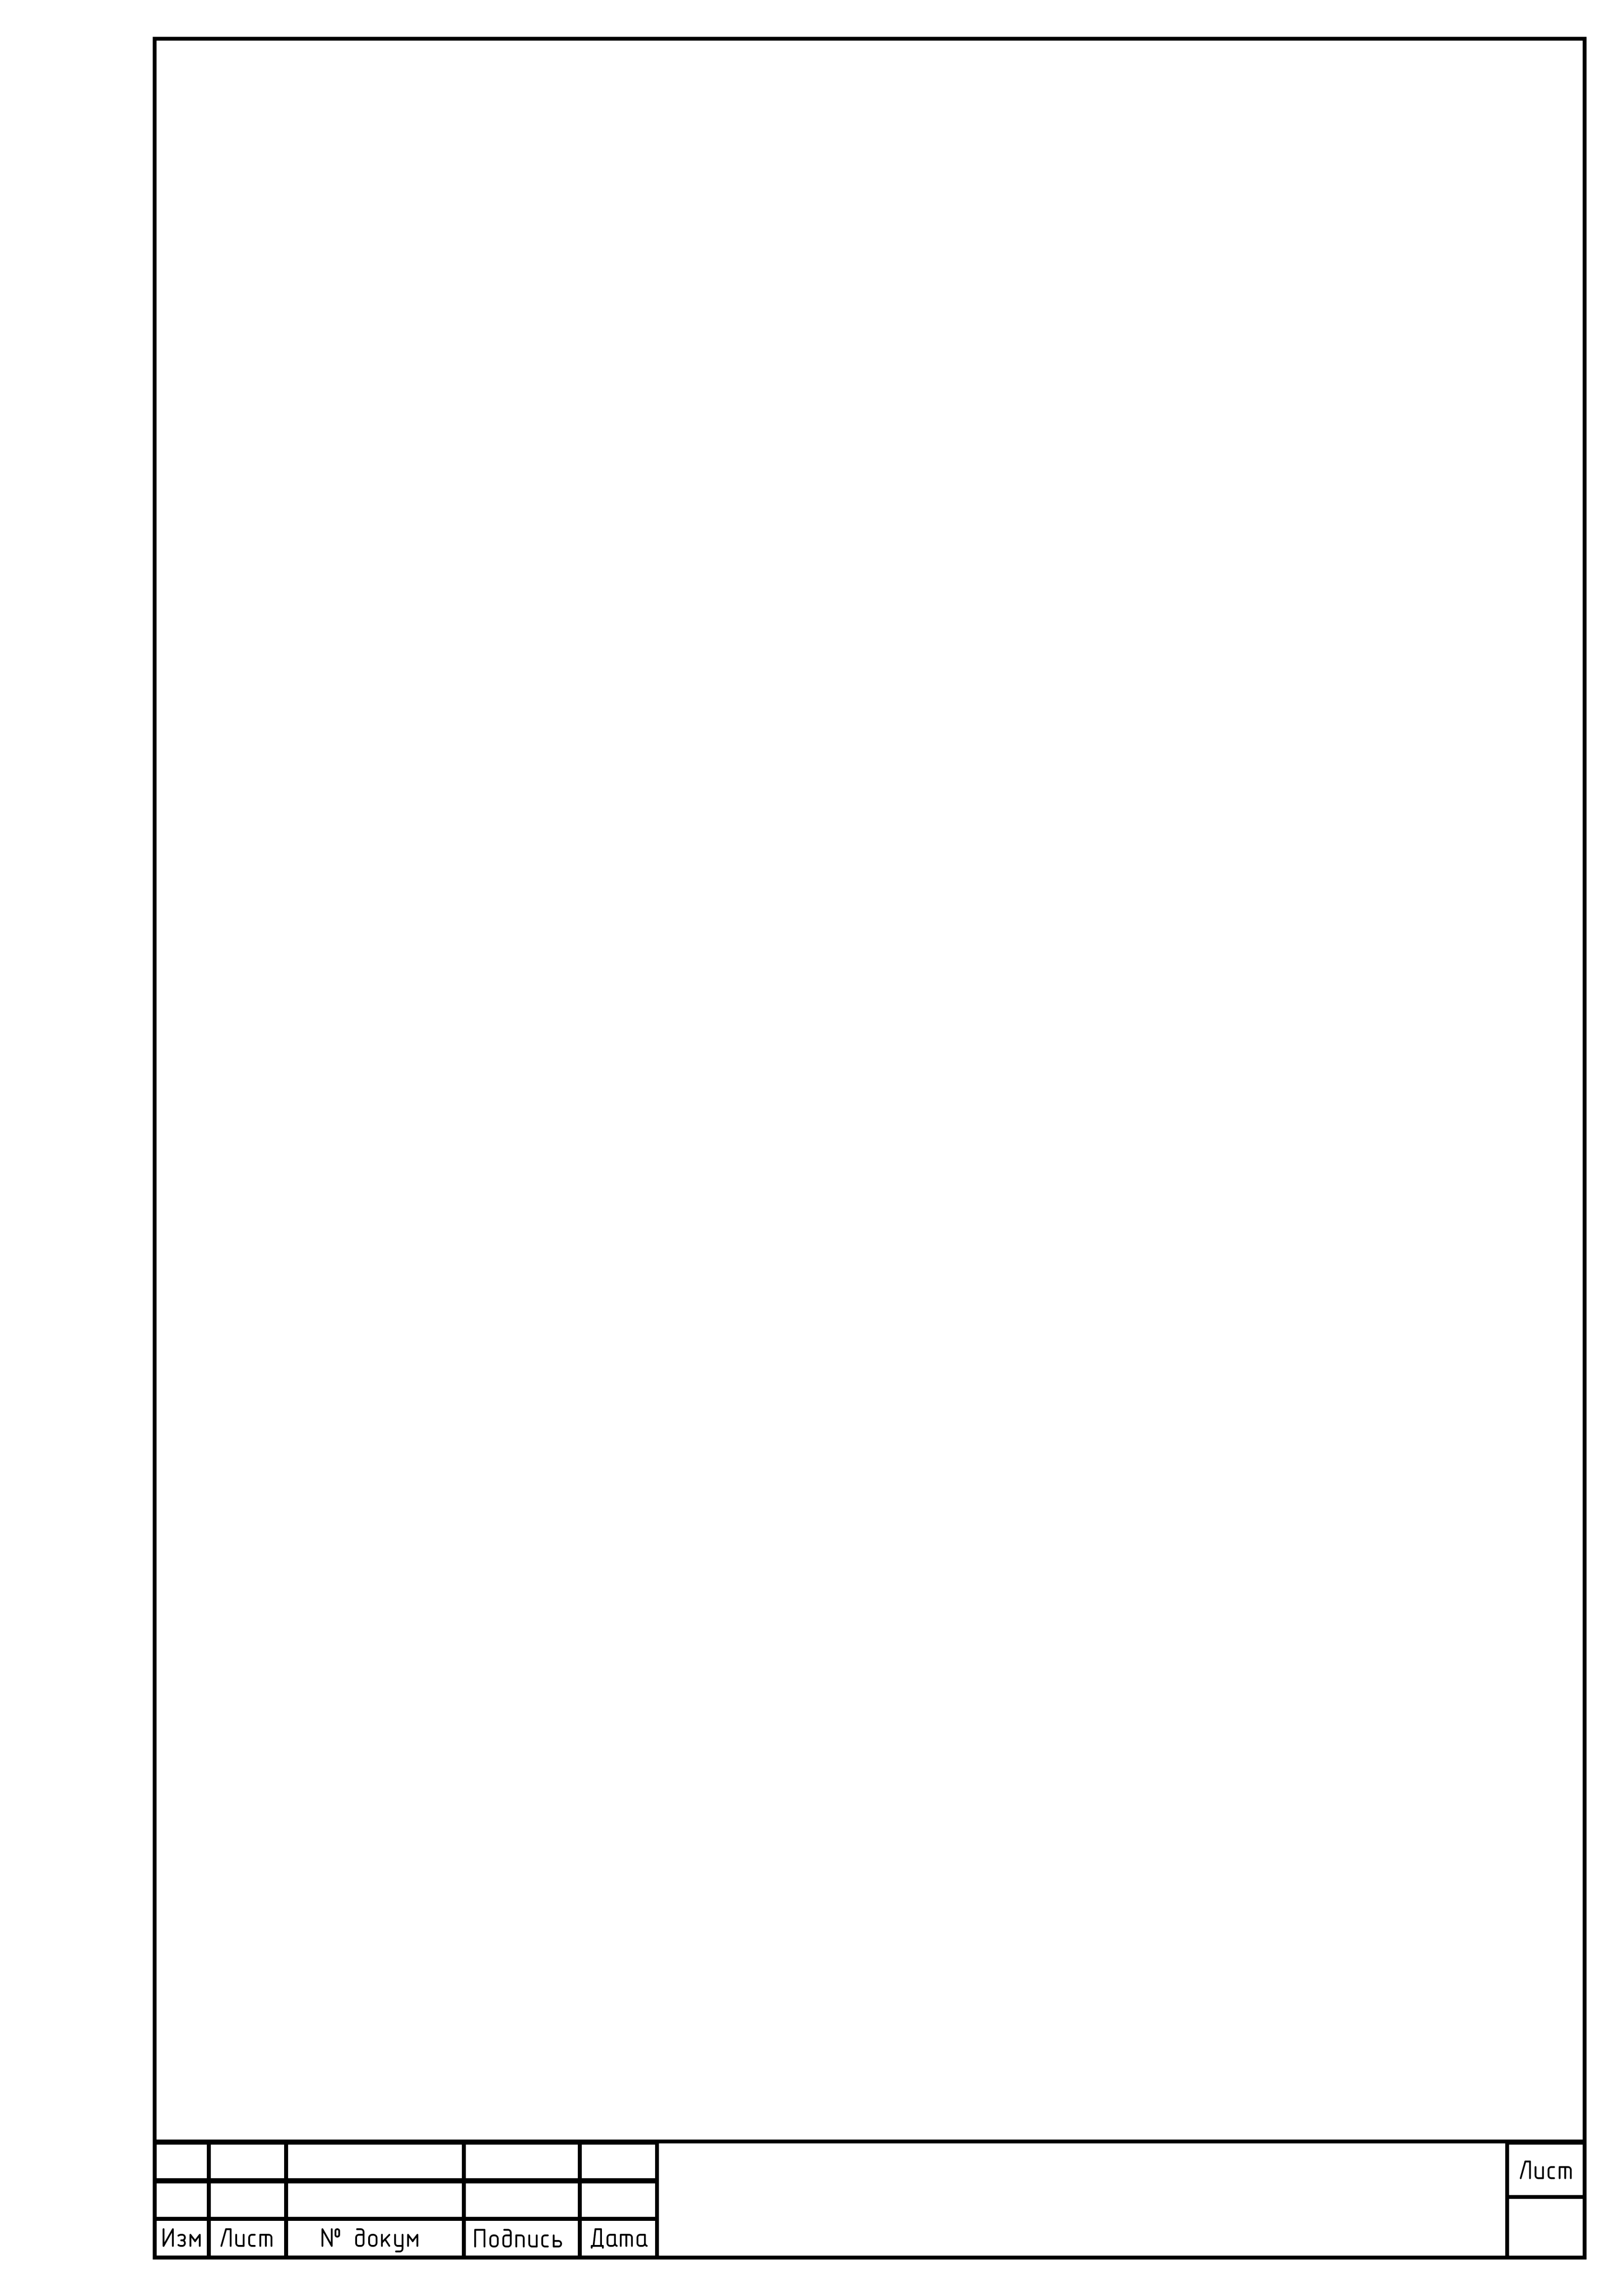
\includegraphics[width=\paperwidth,height=\paperheight]{border/border11.png}}
    }
        \content
    
\end{document}
